\documentclass[12pt, addpoints, answers]{exam}
\usepackage[spanish]{babel}
\usepackage{amsmath}
\usepackage{amssymb}
\usepackage{graphicx}
\usepackage{tabularx}
\usepackage{ragged2e}
\usepackage{geometry}
\usepackage{booktabs}\pointpoints{punto}{puntos}
\usepackage{tikz} % <--- ¡AÑADIDO PARA DIBUJAR EL GRID!
\usetikzlibrary{calc} % Útil para calcular coordenadas exactas

% --- AJUSTE DE MARGENES ---
\geometry{
	hmargin={1in, 1in},
	vmargin={1.2in, 1in},
}
% --- CONFIGURACIÓN DE PÁGINA Y ENCABEZADO FINAL ---
\pagestyle{headandfoot}
% 1. Definición Ultra-Robusta del Encabezado (soluciona Overfull \hbox)
\renewcommand{\thepart}{\alph{part}}
\renewcommand{\firstpageheadrule}{%
	\dimen0=\tabcolsep
	\makebox[\textwidth]{%
		\hspace{-\dimen0}\makebox[\textwidth+2\dimen0]{%
			\textbf{Nombre del estudiante:} \enspace\hrulefill \hspace{2em}
			\textbf{Grupo:} \enspace\hrulefill
		}%
	}\vspace{1ex}\hrule
}
\renewcommand{\solutiontitle}{\textbf{Solución:}} %Este nuevo comando sustituye solution por solución: pregunta 18
% 2.  Se define el contenido del encabezado de la universidad (centrado)
\firstpageheader{}{\centering\textbf{Examen Diagnóstico de Matemática. Batería 2}\\\textbf{Universidad Estatal Guayaquil}}{}

% 3. Define el pie de página
\firstpagefooter{}{Página \thepage\ de \numpages}{}
\runningheader{Diagnóstico Matemática}{}{Pág. \thepage}
\runningfooter{}{}{}
\newcommand{\tf}[1]{\fillin[#1][0.25in]}

\begin{document}
	
	% --- NUEVA SECCIÓN PARA DATOS DEL ALUMNO ---
	% Usamos \makebox para alinear el Nombre a la izquierda y el Grupo a la derecha.
	\makebox[\textwidth]{
		\textbf{Nombre:} \enspace\hrulefill \hspace{4em}  
		\textbf{Grupo:} \enspace\hrulefill 
	}
	
	
	
	\vspace{1 cm}
	
		% COMIENZA EL EXAMEN (Todas las preguntas)
	\begin{questions}
	\question[1] \textbf{	Considerando las siguientes funciones, calcula sus respectivas imágenes para $x = -1$; $x = 0 $; $x = 1 $; $x =\sqrt{2}$ }
		\begin{parts}
		\part $f(x)=4x^2 + 2 $
		\part $g(x)= -2x^{2}+2$
		\part $h(x)=\sqrt{2} - 2x^{2}$
		\part $k(x)=5+2^{x-2}$
		\end{parts}
		\question[1] \textbf{Determina si las siguientes funciones son inyectivas.}
		\begin{parts}
		\part $f(x)=5x+\frac{1}{2}$
		\part $g(x)=-4x^{2}+6$
		\part $h(x)=\sqrt{x}-3$
		\part $k(x)=x^{2}+1$
		\end{parts}
\question[1] \textbf{Dadas las siguientes funciones $g(x)=4x^{2}+\dfrac{1}{2}$  y   $f(x)=5x^{2}-\dfrac{1}{2}$. Calcule.}
 \begin{parts}
		\part $f(x)+g(x)$
		\part $f(x)-g(x)$
		\part $(g\circ f)$
		\part $\frac{g(x)}{f(x)}$
		\end{parts}
\question[1]\textbf{De la función $f(x)=x^{2}-2x-8$ diga cuáles son sus raíces:}
 \begin{parts}
		\part$x_{1}=2$ $x_{2}=4$
		\part$x_{1}=-2$ $x_{2}=-4$
		\part$x_{1}=-2$ $x_{2}=4$
		\part$x_{1}=-2$ $x_{2}=2$
		\end{parts}
\question[1]\textbf{Asocia cada función con su gráfica.}
 \begin{parts}
		\part $f(x)=\log_2(x)$
		\part $g(x)=5$
		\part $h(x)= \left| \frac{1  }{2}x+5 \right|$
		\part $k(x)=-\dfrac{1}{2}x+5$
		\part $m(x)=x^{2}-2x-8$
		\part $n(x)=2^{x}$
		\part $p(x)=2x$
		\part $q(x)=-x^{2}-2x+8$
		\end{parts}
		
\vspace{1in}
\noindent % Aseguramos que la minipage se pegue al margen
% primeros fila de 4 gráficos
\begin{minipage}[t]{0.23\linewidth}
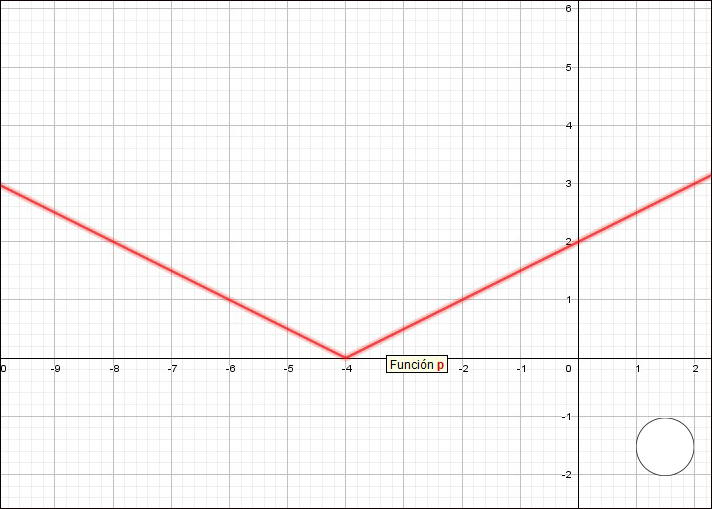
\includegraphics[width=1\linewidth]{Figuras/fig1}
\end{minipage}\hfill
\begin{minipage}[t]{0.23\linewidth}
	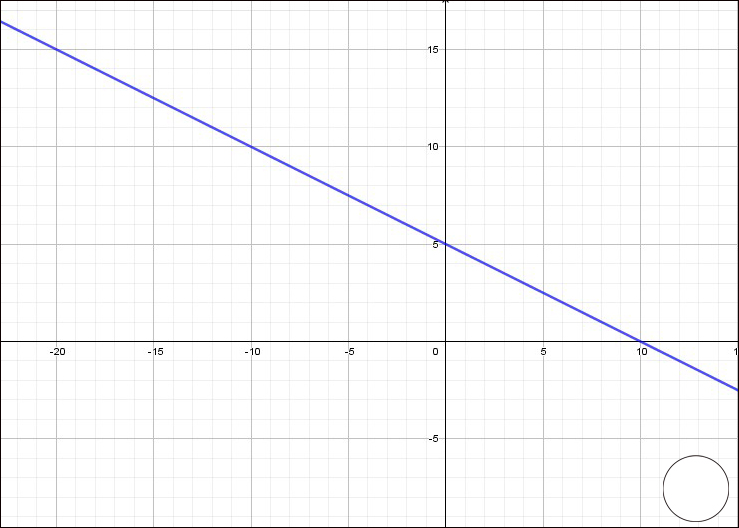
\includegraphics[width=1\linewidth]{Figuras/fig2}
\end{minipage}\hfill
\begin{minipage}[t]{0.23\linewidth}
	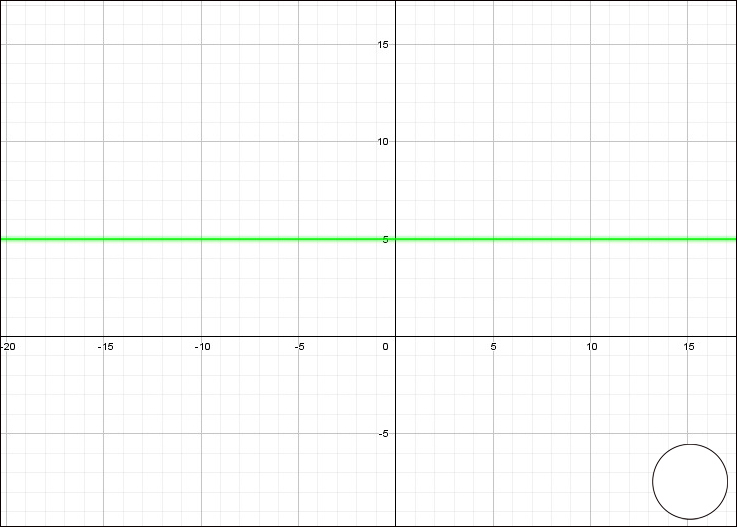
\includegraphics[width=1\linewidth]{Figuras/fig3}
\end{minipage}\hfill
\begin{minipage}[t]{0.23\linewidth}
	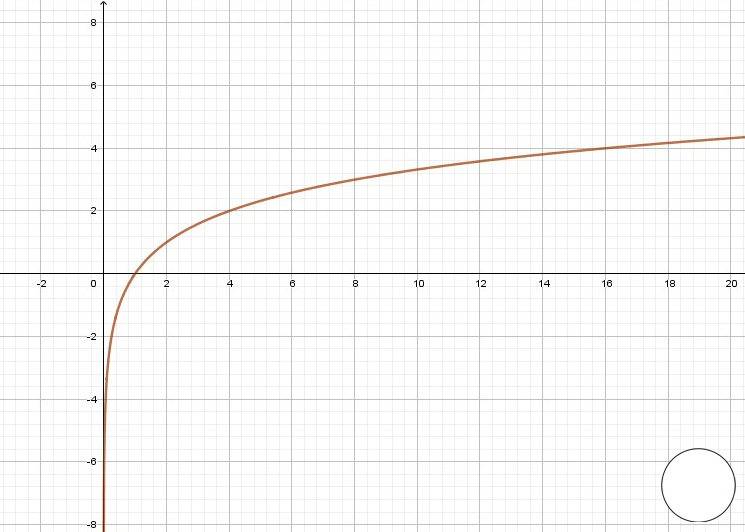
\includegraphics[width=1\linewidth]{Figuras/fig4}
\end{minipage}
\par\vspace{1cm} % Se agrega el comando \par para asegurar  un salto de línea  garantizando transición al modo vertical.			
\noindent		
\begin{minipage}[t]{0.23\linewidth}	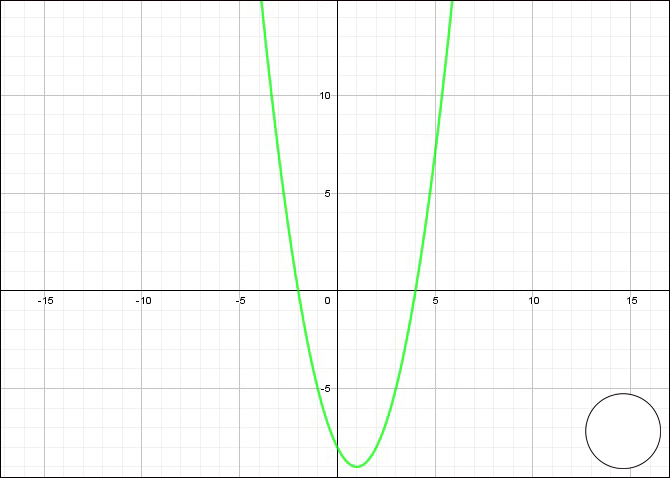
\includegraphics[width=1\linewidth]{Figuras/fig5}
\end{minipage}\hfill	
\begin{minipage}[t]{0.23\linewidth}
	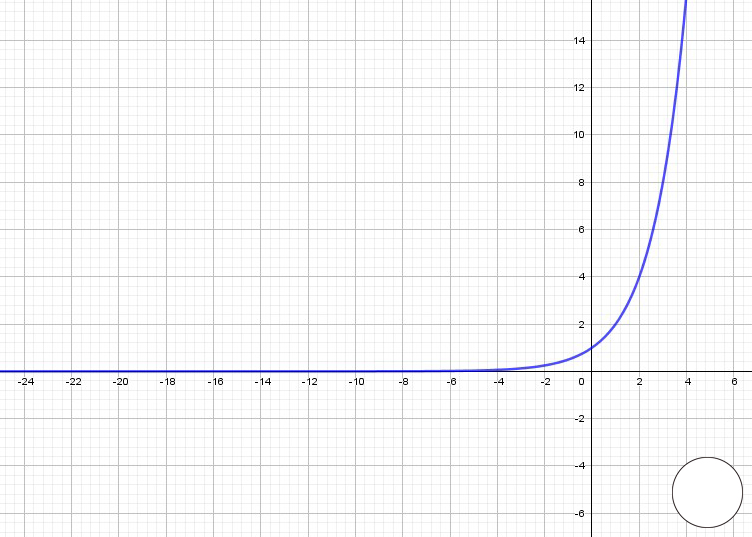
\includegraphics[width=1\linewidth]{Figuras/fig6}
\end{minipage}\hfill		
\begin{minipage}[t]{0.23\linewidth}
	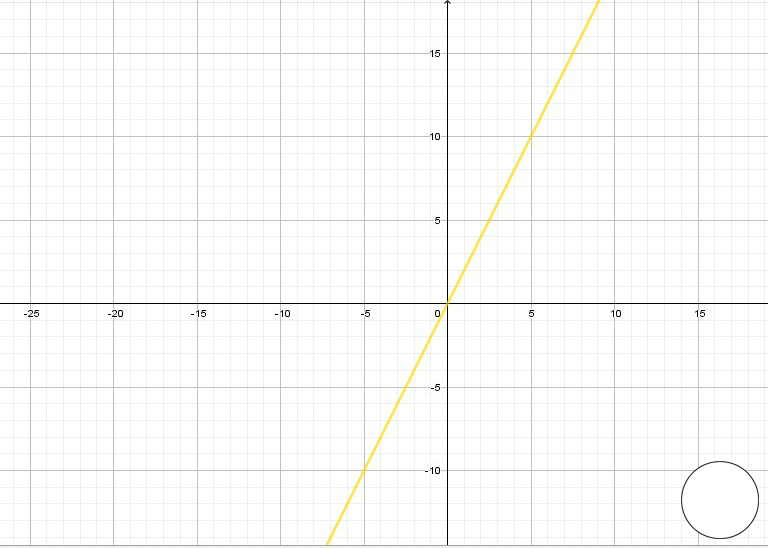
\includegraphics[width=1\linewidth]{Figuras/fig7}
\end{minipage}\hfill	
\begin{minipage}[t]{0.23\linewidth}
	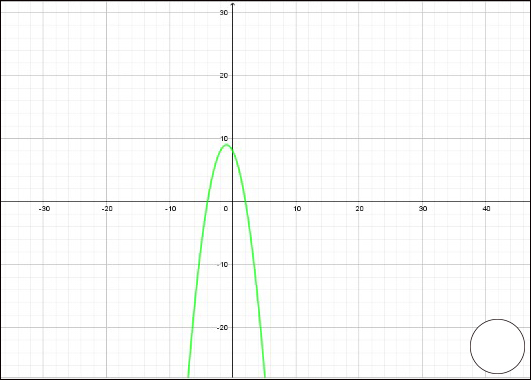
\includegraphics[width=1\linewidth]{Figuras/fig8}
\end{minipage}
\par\vspace{0.5cm}
\question[1]\textbf{Asocia cada ecuación de la circunferencia con su gráfica correspondiente.}	
    \begin{parts}
    \part $(x+4)^{2}+(y-4)^{2}=16$	
     \part $(x-1)^{2}+(y-1)^{2}=1$
      \part $(x-4)^{2}+(y+2)^{2}=4$	
       \part $(x+1)^{2}+(y+1)^{2}=1$
         
    \end{parts}	
\par\vspace{0.5cm}
\noindent 
\begin{minipage}[t]{0.23\linewidth}
	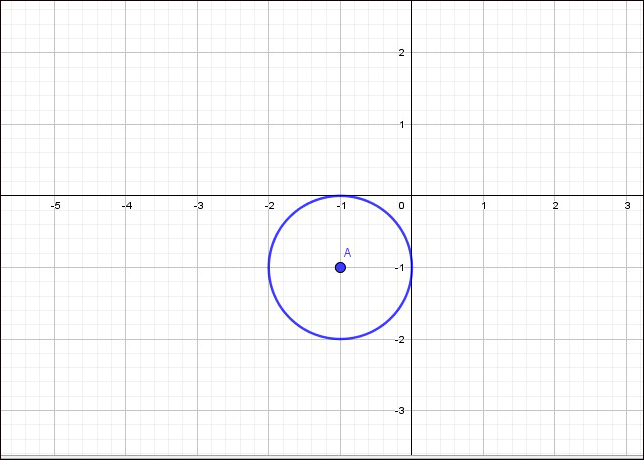
\includegraphics[width=1\linewidth]{Figuras/fig9}
\end{minipage}\hfill
 \begin{minipage}[t]{0.23\linewidth}
 	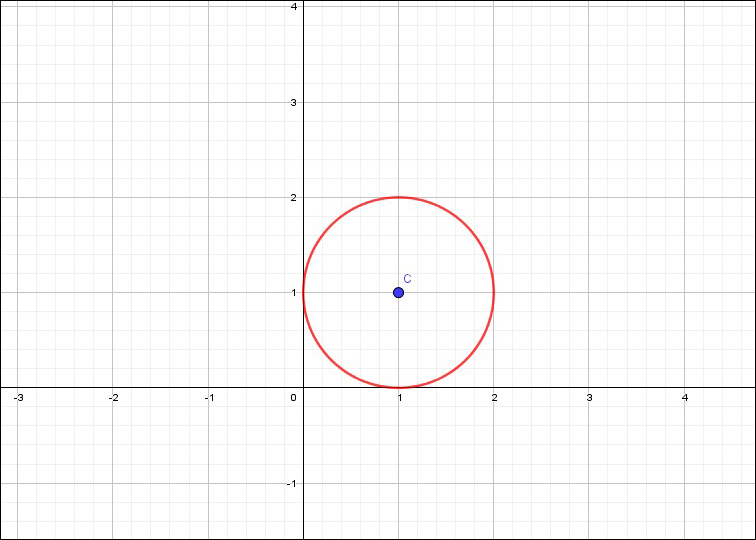
\includegraphics[width=1\linewidth]{Figuras/fig10}
 \end{minipage}\hfill
 \begin{minipage}[t]{0.23\linewidth}
 	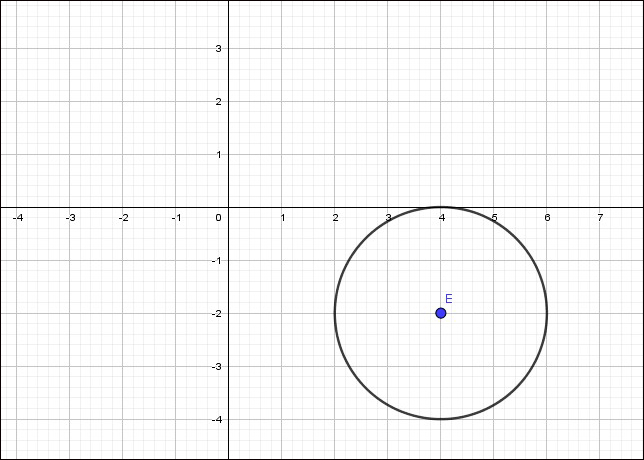
\includegraphics[width=1\linewidth]{Figuras/fig11}
 \end{minipage}\hfill 
 \begin{minipage}[t]{0.23\linewidth}
 	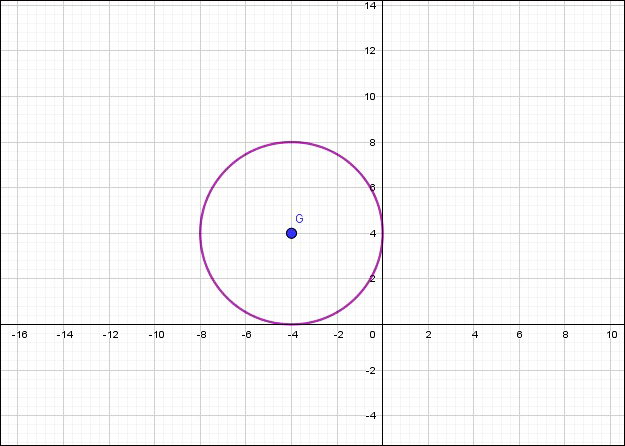
\includegraphics[width=1\linewidth]{Figuras/fig12}
 \end{minipage} 
\question[1] \textbf{Calcula el valor de los siguientes límites}.
    \begin {parts}
        \part$\lim\limits_{x \to -4} \left| x+4 \right|$
        \part $\lim\limits_{x \to 2} \frac{\left| x-2 \right|}{x-3}$
        \part $\lim\limits_{x \to 2} \frac{x^2 - 5x + 6}{x^2 + 3x - 10}$
        \part $\lim\limits_{x \to \infty} \frac{4}{x}$
        \end {parts}
 \question[1]\textbf{Deriva las funciones siguientes utilizando las reglas de derivación básicas.}
            \begin{parts}
        	\part$f(x)=-5x^{2}+8$
        	\part$f(x)=-5\pi^{3}$
        	\part$f(x)=-12x^{2}+8x+15$
        	\part $f(x)=-20x^{2}+\sqrt{12}$
        \end{parts}
        
\question[1] \textbf{Si $f$ es una función de  $ \mathbb{R}$ en $\mathbb{R}$  tal que $f(x)=x^{2}+x$, se puede afirmar que:\textit{(Dibuje la función $f(x)$ en el espacio en blanco de la derecha)}} 
 \begin{parts} 
	\part$f$ es una función par.	
	\part$f$ es una función inyectiva.
	\part$ rgf= [0,+\infty)$
	\part$\forall x \in \mathbb{R}$, $f$ es creciente.
	\part$ f $ decrece en$(-\infty,-1]$.	%Esta es la respuesta correcta	
 \end{parts}
 % --- PREGUNTA 10: FUNCIÓN A TROZOS CON GRID DE TIKZ ---
\question[1] \textbf{Grafique la siguiente función definida por partes en la cuadrícula provista:}

% Definición de la Función a Trozos
\begin{equation*}
	f(x)=
	\begin{cases} 
		-x-2 & \text{si } x < -2 \\
		4 & \text{si } -2 \le x < 1 \\
		\frac{x}{2}+\frac{1}{2} & \text{si } x \ge 1
	\end{cases}
\end{equation*}

\par\vspace{0.5em}

\noindent
\begin{center}
	
	
	\shorthandoff{>} % Necesario por conflicto entre babel/spanish y tikz/flechas
	\begin{tikzpicture}[scale=0.8] 
		
		% 1. Definición del Grid: -5 a 5 con paso de 5mm (0.5cm)
		\def\step{0.5} 
		\def\minCoord{-5} \def\maxCoord{5}
		
		% Dibujar la cuadrícula de 5mm (gris claro)
		\draw[step=\step cm, gray!50, very thin] (\minCoord, \minCoord) grid (\maxCoord, \maxCoord);
		
		% 2. Ejes Coordenados (gruesos con flechas)
		\draw[->, thick] (\minCoord-0.5, 0) -- (\maxCoord+0.5, 0) node[right] {$x$};
		\draw[->, thick] (0, \minCoord-0.5) -- (0, \maxCoord+0.5) node[above] {$f(x)$};
		
		% 3. Marcas de Ticks y etiquetas (cada 1 unidad)
		\foreach \x in {-4, -3, -2, -1, 1, 2, 3, 4}
		\draw (\x, 0.1) -- (\x, -0.1) node[below] {\footnotesize $\x$};
		
		\foreach \y in {-4, -3, -2, -1, 1, 2, 3, 4}
		\draw (0.1, \y) -- (-0.1, \y) node[left] {\footnotesize $\y$};
		
		% Centro 0
		\node at (0.25, -0.25) {\footnotesize 0};
		
		% NOTA: NO SE DIBUJAN LAS FUNCIONES (Grid vacío)
		
	\end{tikzpicture}
	\shorthandon{>} % Reactivar shorthand
\end{center}
\question[1] \textbf{Al simplificar la expresión algebraica: }
\begin{equation*}
	\frac{(2x^{n+1})^{2} \cdot x^{3-n}}{x^{2(n+1)}(x^{n})^{2}}
\end{equation*}
\textbf{se obtiene:}
\begin{oneparcheckboxes}
\choice $4x^{n+3}$
\choice $4x^{n-3}$
\choice $4x^{3-3n}$ % Esta es la solución del ejercicio
\choice $4x^{n}$
\choice $4x^{3n+1}$	
\end{oneparcheckboxes}
\question[1] Una población de bacterias crece de tal manera que cada día hay el doble de las que había el día anterior. Si en el día diez se encontraron 1024 bacterias, entonces en el primer día había:

\begin{oneparcheckboxes}
	\choice 4 bacterias
	\choice 6 bacterias
	\choice 1 bacteria
	\choice 2 bacterias % respuesta correcta
	\choice 3 bacterias
\end{oneparcheckboxes}
\question[1]Sea $L$ la recta que contiene los puntos $P_{1}(2,0 )$ y $P_{2}(0,4)$
Entonces es \textbf{verdad} que:
\begin{parts} 
	\part La pendiente de $L$ es menor que -2.	
	\part$(3,3)$ $\in$ a $L$.
	\part$L$ es paralela a la recta $y=-2x$ % Respuesta correcta
	\part La distancia de $L$,al origen de coordenadas es menor que 1.
	\part$L$ es perpendicular a la recta $y=2x$.		
\end{parts}
\question[1] Escriba  Verdadero o Falso.

 \tf{} Toda función $f:  \mathbb{R} \rightarrow \mathbb{R}$ estrictamente creciente es sobreyectiva. % Falso contraejemplo $f(x)=2^{x}
   
\tf{} Si $f$ es una función de $\mathbb{R}$ en $\mathbb{R}$ tal que $f(x)=a^{x}$, con $a \in \mathbb{R}^{+}$ -\{1\}, entonces $f(x+y)=f(x) \cdot f(y)$. % Verdadera
 
\tf{} El número $\frac{\pi}{2\pi}+4$ es irracional. %Falso

\tf{}$\log_{2}{3}$=$\frac{1}{\log_{3}{2}}$ %Verdadero, aplicar cambio de base

\question[1] Los valores reales de x que satisfacen la desigualdad $1-x\geq2x+6$ son:
\begin{oneparcheckboxes}
	\choice $x\geq \frac{-5}{3}$
	
	\choice $x\leq\frac{5}{3}$
	
	\choice $x\geq\frac{2}{3}$ 
	
	\choice $x\leq\frac{-5}{3}$ % respuesta correcta

\end{oneparcheckboxes}

\question[1] Sean $f:\mathbb{R} \rightarrow \mathbb{R}$ y $g:\mathbb{R} \rightarrow \mathbb{R}$ dos funciones tales que $f(x)=x$ y $g(x)=x ^{2}$, entonces es VERDAD que:
\begin{parts} 
	\part $f+g$ es una función inyectiva.	
	\part$f-g$ es una función sobreyectiva.
	\part $f\cdot g$ Es una función sobreyectiva % respuesta correcta
	\part$\frac{g}{f}$ está definida para todo valor de$x$ 
	\part $\frac{f}{g}$	es una función lineal.	
\end{parts}
% Asegúrese de que los siguientes paquetes están incluidos en su preámbulo:
% \usepackage{amsmath}
% \usepackage{amssymb}
% \usepackage{tikz}
% \usepackage[spanish]{babel}

\question[2] \textbf{Determina la ecuación de cada uno de los gráficos que se muestran a continuación:}
\par\vspace{0.5em}

% Definiciones generales para los gráficos (rango de [-5, 5])
\def\minC{-5} \def\maxC{5}
\def\step{0.5}

\noindent
\begin{minipage}[t]{0.48\linewidth}
	\centering %\textbf{(a)} $f(x)=3^{x}+C$
	\shorthandoff{>}
	\begin{tikzpicture}[scale=0.6] 
		% 1. Grid (0.5cm)
		\draw[step=\step cm, gray!50, very thin] (\minC, \minC) grid (\maxC, \maxC);
		% 2. Ejes
		\draw[->, very thick] (\minC-0.5, 0) -- (\maxC+0.5, 0) node[right] {$x$};
		\draw[->, very thick] (0, \minC-0.5) -- (0, \maxC+0.5) node[above] {$y$};
		% 3. Ticks (Números más pequeños: \tiny)
		\foreach \x in {-4, -3, -2, -1, 1, 2, 3, 4} \draw (\x, 0.1) -- (\x, -0.1) node[below] {\tiny $\x$};
		\foreach \y in {-4, -3, -2, -1, 1, 2, 3, 4} \draw (0.1, \y) -- (-0.1, \y) node[left] {\tiny $\y$};
		\node at (0.25, -0.25) {\tiny 0};
		
		% 4. Función: y=3^x - 3 (Verde, very thick)
		\draw[domain=-2:1.5, samples=100, smooth, very thick, green!70!black] plot (\x, {3^(\x) - 3});
		
		% 5. Asíntota: y=-3 (Rojo, Discontinua)
		\draw[red, dashed, thick] (\minC, -3) -- (\maxC, -3);
		
		% 6. Etiqueta
		\node[anchor=south east, font=\small, text=black] at (4.8, 4.8) {$f(x)=3^{x}+C$};
	\end{tikzpicture}
	\shorthandon{>}
\end{minipage}\hfill
\begin{minipage}[t]{0.48\linewidth}
	\centering %\textbf{(b)} $f(x)=10^{x+b}$
	\shorthandoff{>}
	\begin{tikzpicture}[scale=0.6]
		% 1. Grid (0.5cm)
		\draw[step=\step cm, gray!50, very thin] (\minC, \minC) grid (\maxC, \maxC);
		% 2. Ejes
		\draw[->, very thick] (\minC-0.5, 0) -- (\maxC+0.5, 0) node[right] {$x$};
		\draw[->, very thick] (0, \minC-0.5) -- (0, \maxC+0.5) node[above] {$y$};
		% 3. Ticks (Números más pequeños: \tiny)
		\foreach \x in {-4, -3, -2, -1, 1, 2, 3, 4} \draw (\x, 0.1) -- (\x, -0.1) node[below] {\tiny $\x$};
		\foreach \y in {-4, -3, -2, -1, 1, 2, 3, 4} \draw (0.1, \y) -- (-0.1, \y) node[left] {\tiny $\y$};
		\node at (0.25, -0.25) {\tiny 0};
		
		% 4. Función: y=10^(x-1) (Rojo, very thick)
		\draw[domain=-0.5:1.5, samples=100, smooth, very thick, red!80!black] plot (\x, {10^(\x-1)});
		
		% 5. Punto A=(1,1) (Azul) - Coordenadas movidas al primer cuadrante
		\fill[blue] (1, 1) circle (2.5pt) node[anchor=south west, font=\small, blue] {A (1, 1)};
		
		% 6. Etiqueta
		\node[anchor=south east, font=\small, text=black] at (4.8, 4.8) {$f(x)=10^{x+b}$};
	\end{tikzpicture}
	\shorthandon{>}
\end{minipage}

\par\vspace{1em} % Salto de línea entre filas de gráficos

\noindent
\begin{minipage}[t]{0.48\linewidth}
	\centering %\textbf{(c)} $f(x)=a^{x+b}+C$
	\def\minCx{-2} \def\maxCx{8}
	\def\minCy{-5} \def\maxCy{5}
	\shorthandoff{>}
	\begin{tikzpicture}[scale=0.45] 
		% 1. Grid (0.5cm)
		\draw[step=\step cm, gray!50, very thin] (\minCx, \minCy) grid (\maxCx, \maxCy);
		% 2. Ejes
		\draw[->, very thick] (\minCx-0.5, 0) -- (\maxCx+0.5, 0) node[right] {$x$};
		\draw[->, very thick] (0, \minCy-0.5) -- (0, \maxCy+0.5) node[above] {$y$};
		% 3. Ticks (Números más pequeños: \tiny)
		\foreach \x in {-1, 1, 2, 3, 4, 5, 6, 7} \draw (\x, 0.1) -- (\x, -0.1) node[below] {\tiny $\x$};
		\foreach \y in {-4, -3, -2, -1, 1, 2, 3, 4} \draw (0.1, \y) -- (-0.1, \y) node[left] {\tiny $\y$};
		\node at (0.25, -0.25) {\tiny 0};
		
		% 4. Función: y=2^(x-6) - 2 (Azul, very thick)
		\draw[domain=0:8, samples=100, smooth, very thick, blue!70!black] plot (\x, {2^(\x-6) - 2});
		
		% 5. Asíntota: y=-2 (Rojo, Discontinua)
		\draw[red, dashed, thick] (\minCx, -2) -- (\maxCx, -2);
		
		% 6. Punto B=(6,-1) (Azul) - Coordenadas movidas al cuarto cuadrante
		\fill[blue] (6, -1) circle (3.5pt) node[anchor=north west, font=\small, blue] {B (6, -1)};
		
		% 7. Etiqueta (Se mantiene en el primer cuadrante)
		\node[anchor=north east, font=\small, text=black] at (\maxCx-0.2, \maxCy-0.2) {$f(x)=a^{x+b}+C$};
	\end{tikzpicture}
	\shorthandon{>}
\end{minipage}\hfill
\begin{minipage}[t]{0.48\linewidth}
	\centering %\textbf{(d)} $f(x)=C+10^{x+b}$
	% Rango ajustado a Y en [-1, 7]
	\def\minCd{-5} \def\maxCd{5}
	\def\minCyd{-1} \def\maxCyd{7}
	\shorthandoff{>}
	\begin{tikzpicture}[scale=0.6]
		% 1. Grid (0.5cm)
		\draw[step=\step cm, gray!50, very thin] (\minCd, \minCyd) grid (\maxCd, \maxCyd);
		% 2. Ejes
		\draw[->, very thick] (\minCd-0.5, 0) -- (\maxCd+0.5, 0) node[right] {$x$};
		\draw[->, very thick] (0, \minCyd-0.5) -- (0, \maxCyd+0.5) node[above] {$y$};
		% 3. Ticks (Números más pequeños: \tiny)
		\foreach \x in {-4, -3, -2, -1, 1, 2, 3, 4} \draw (\x, 0.1) -- (\x, -0.1) node[below] {\tiny $\x$};
		\foreach \y in {1, 2, 3, 5, 6, 7} \draw (0.1, \y) -- (-0.1, \y) node[left] {\tiny $\y$};
		\draw (0.1, -1) -- (-0.1, -1) node[left] {\tiny $-1$};
		\draw (0.1, 4) -- (-0.1, 4) node[left] {\tiny $4$}; % Ticks del eje Y
		\node at (0.25, -0.25) {\tiny 0};
		
		% 4. Función: y=4 + 10^(x+2) (Rojo, very thick)
		\draw[domain=-5:-1.7, samples=100, smooth, very thick, red!80!black] plot (\x, {4 + 10^(\x+2)});
		
		% 5. Asíntota: y=4 (Rojo, Discontinua)
		\draw[red, dashed, thick] (\minCd, 4) -- (\maxCd, 4);
		
		% 6. Punto C=(-2,5) (Azul) - Coordenadas añadidas
		\fill[blue] (-2, 5) circle (2.5pt) node[anchor=south east, font=\small, blue] {C (-2, 5)};
		
		% 7. Etiqueta (Se mantiene en el primer cuadrante)
		\node[anchor=north east, font=\small, text=black] at (\maxCd-0.3, \maxCyd-0.1) {$f(x)=C+10^{x+b}$};
	\end{tikzpicture}
	\shorthandon{>}
\end{minipage}
\question[1]El gráfico siguiente representa una función del tipo $f(x)=\log_a(x+b)+C$.
\begin{enumerate}
	\item Escribe su ecuación
	\item Determine los valores de x para los que está definida la función.
	\item Halla su cero.
	\item Escribe las coordenadas de los puntos $P_{1},P_{2},P_{3}$ si sus ordenadas son 2,-1 y $\frac{1}{2}$ respectivamente.
	\item Escribe las coordenadas de los puntos $Q_{1},Q_{2},Q_{3}$ si sus absisas son 25,$\frac{-5}{3}$, y 0 respectivamente.
	\end{enumerate}
\begin{solution}
	\begin{enumerate}
		\item $f(x)=$ % Respuesta\longrightarrow $f(x)=\log_3(x+24)-2$
		\item Dominio= % x\in R/x > -24
		\item $x=$ % x=-15
		\item $P_{1}=$\hspace{1in}$P_{2}=$\hspace{1in}$P_{3}=$ % p1=(57,2)   p2=(-21,-1)   p3=(-8.41,0.5)
		\item $Q_{1}=$\hspace{1in}$Q_{2}=$\hspace{1in}$Q_{3}=$ % q1=(25,1.59) q2=(-5/3,0.85)  p3=(0,0.89)
	\end{enumerate}
\end{solution}

\begin{center}
	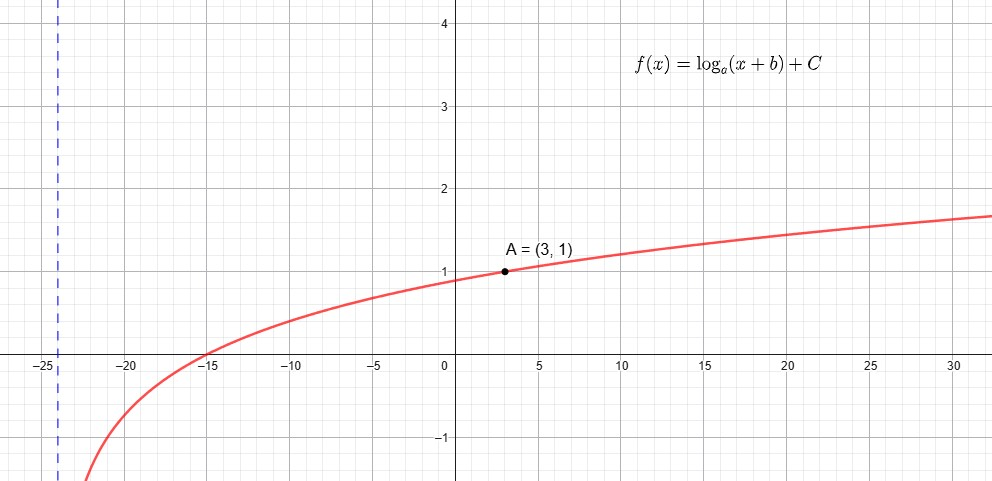
\includegraphics[width=0.7\linewidth]{Figuras/fig13}
\end{center}
\vspace{0.5 cm}
\question[1]\textbf{Resuelve las siguientes ecuaciones.}
\begin{enumerate}
	\item $\log_3(x+4)+\log_3(x-4)=2$ % Solución x=5, x=-5
	\item $\log_2(x-8)-\log_2(x+6)=3$ % solución: x=-8 
	\item $ 2\log_7(x)=\log_7(3x)+\log_7(6)$ %solución: x=0, x=18
	\item $ \log_2(x+7)-\log_2(x-11)=2$
	
	\begin{solution}
		\begin{enumerate}
			\item $x_{1}= \hspace{0.8in} x_{2}=$
			\item $x_{1}= $
				\item $x_{1}= \hspace{0.8in} x_{2}=$
					\item $x_{1}= \hspace{0.8in} x_{2}=$
		\end{enumerate}
	\end{solution}
\end{enumerate}
\question[1] \textbf{¿Cuáles de las proposiciones siguientes son falsas (F) o verdaderas (V)?}
 
\tf{} En un triángulo al mayor ángulo se opone el mayor lado.

\tf{} Todo triángulo isósceles es equilátero.

\tf{} En un triángulo, la altura relativa a uno de sus lados pasa por el punto medio.

\tf{} En un triángulo rectángulo e isósceles, la longitud de la altura correspondiente a la hipotenusa es igual a la mitad de la longitud de esta.

\tf{} Es posible construir un triángulo con tres segmentos que midan 5,12,4 cm. %Falso. No se cumple la desigualdad triangular para los lados 5+4>9

\tf{} Un triángulo tiene 3 m más de altura que de base y su área es de 20 $m^{2}$   Sus  dimensiones son: Base=5m, Altura=8m % verdadero 

\tf{} En un triángulo rectángulo, los ángulos agudos miden $2x+30^\circ$ y $3x+15^\circ$ respectivamente. Dichos ángulos miden 48$^\circ$ y 52$^\circ$ %Falso los angulos miden 48 y 42









\end{questions}	

\end{document}